\chapter{Theoretical Background}

This chapter will give a brief overview about the underlying theoretical background in the fields of antenna theory, spatial sampling, will introduce some methods of integration to derive the \ac{TRP} out of spherical \ac{EIRP}-data and will establish the needed stochastic for the used statistic.

\section{Antenna Field Regions}

\begin{figure}[H]
\centering
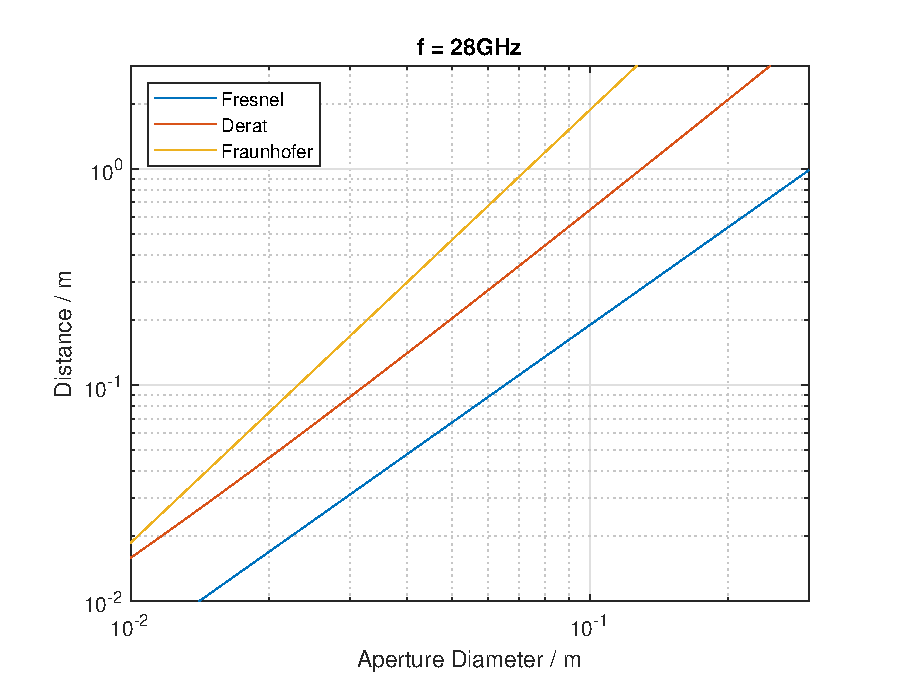
\includegraphics[width=0.6\textwidth]{Matlab/AntennaFieldRegions.eps}
\caption{Antenna field regions overview}
\label{fig:antennafieldreg}
\end{figure}

There are three commonly known antenna regions, the reactive \ac{NF}, the radiating \ac{NF} and the \ac{FF}, divided by two boundaries, the Fresnel distance (blue) and the Fraunhofer distance (yellow). These distances are shown in figure \ref{fig:antennafieldreg}, where the aperture diameter of an arbitrary antenna is on the x-axis and the distance form it is on the y-axis. The third line, the Derat distance (red) was introduced by Benoit Derat in \cite{8393926}.\\
\ac{FF}-distance and \ac{NF}-distance are derivable from the phase fluctuation due to the maximum diameter of the antennas aperture \cite{7942128} in a distance $r$ from the antennas phase center. The phase fluctuation is given by the different length of $r$ and $R$, as you can see in figure \ref{fig:arbaperturexy}. The maximum runtime difference is found at the minimum radius of the circle enclosing the aperture at $\sfrac{D}{2}$. The field boundaries are derived from the Taylor series of the function of the phase in dot $P$. Fresnel and Fraunhofer distance, the boundaries between reactive \ac{NF}, radiating \ac{NF} (Fresnel-Region) and the \ac{FF} (Fraunhofer-Region), are analogue to their optical counterpart. \cite{7942128} \cite{balanis}

\begin{figure}[H]
\centering
\def\svgwidth{0.6\textwidth}
\input{Bilder/AntennaApature.pdf_tex}
\caption{An arbitrary radiating aperture in the $yz$ plane. \cite{7942128}}
\label{fig:arbaperturexy}
\end{figure}

$R$ is the distance from an arbitrary point on the aperture to an other arbitrary point $P$ in the volume. With $r$, the distance from the phase center of the antenna to the point $P$, $R$ can be written as: \cite{balanis}

\begin{equation}
R = \sqrt{\left(x^2+y^2+z^2\right)-\left(2zz'-z^{\prime\, 2}\right)}=\sqrt{r^2-\left(2rz'\sin \theta -z^{\prime\, 2}\right)}
\end{equation}

Using the binomial expansion, $R$ can then be rewritten as:

\begin{equation}
R = r - z'\sin\theta + \frac{1}{r}\left(\frac{z^{\prime\, 2}}{2}\cos ^2 \theta\right) + \frac{1}{r^2}\left(\frac{z^{\prime\, 3}}{2}\sin\theta\cos^2\theta\right) + \dots
\end{equation}

\subsection{Far-Field}

According to \cite{balanis} the \ac{FF}-distance is \glqq that region of the field of an antenna where the angular field distribution is essentially independent of the distance from the antenna.\grqq{ }That means that the antenna's pattern is mostly independent from the distance to the antenna.\\
For the \ac{FF} assumption it is convenient to use the two most significant terms of the binomial expansion $R\approx r - z'\sin\theta$. Hence the error of that truncation can be expressed as the maximum of the third most significant term:

\begin{equation}
\frac{1}{r}\left(\frac{z^{\prime\, 2}}{2}\cos ^2 \theta\right)_\text{max} = \frac{z^{\prime\, 2}}{2r} \quad , \quad \theta = 0
\label{eq:dphi1}
\end{equation}

Introducing the angular wavenumber $k=\sfrac{2\pi}{\lambda}$ and $z'=\sfrac{D}{2}$, formula \ref{eq:dphi1} can be written as:


\begin{equation}
\Delta\phi = \frac{k\cdot z^{\prime\, 2}}{2r} =\frac{\frac{2\pi}{\lambda}\cdot \left(\frac{D}{2}\right)^2}{2r} = \frac{\pi D^2}{4\lambda\cdot r}
\end{equation}

With the typically tolerated phase error of $\Delta\phi = \sfrac{\pi}{8} \ \widehat{=}\  22.5^\circ$ the well known \ac{FF}-distance-formula $r_{\text{Fr}}$ can be derived:

\begin{equation}
\frac{\pi}{8} = \frac{\pi D^2}{4\lambda\cdot r_{\text{Fr}}} \quad \Leftrightarrow \quad r_{\text{Fr}} = \frac{2D^2}{\lambda}
\label{eq:ff}
\end{equation}

This equation is valid for $D > \lambda$. \cite{balanis}

\subsection{Near-Field}

The radiating \ac{NF} (Fresnel) -region is defined by \cite{balanis} as \glqq that region of the field of an antenna between the reactive near-field region and the far-field region wherein radiation fields predominate and wherein the angular field distribution is dependent upon the distance from the antenna.\grqq{ }That means that the antennas pattern is dependent from the distance to the antenna.\\
In the radiating \ac{NF} the deviation from the third most significant term is more then $\sfrac{\pi}{8}$, so it is no longer negligible. With the derivation of the next term the maximum deviation is found:

\begin{align}
\frac{\partial}{\partial\theta}\left(\frac{1}{r^2}\left(\frac{z^{\prime\, 3}}{2}\sin\theta\cos^2\theta\right)\right) = \frac{z^{\prime\, 3}}{2r^2}\cos\theta\left(\cos^2\theta-2\sin^2\theta\right) = 0 \quad \Leftrightarrow\\ 
\theta_1 = \frac{\pi}{2},\ \theta_2=2\arctan\left(\sqrt{5-2\sqrt{6}}\right) \quad \Leftrightarrow
\end{align}

By introducing the angular wavenumber $k=\sfrac{2\pi}{\lambda}$, the minimum sphere diameter $D$, so that $z'=\sfrac{D}{2}$ and the phase error of $\Delta\phi = \sfrac{\pi}{8} \ \widehat{=}\  22.5^\circ$ the \ac{NF} (Fresnel)-distance-formula $r_{\text{NF}}$ can be derived:

\begin{equation}
\Delta\phi = \frac{\pi}{8} = \frac{kz^{\prime\, 3}}{2r_{\text{NF}}^2}\sin\theta_2\cos^2\theta_2= \frac{\pi D^3}{12\sqrt{3}\cdot\lambda r_{\text{NF}}^2} \quad \Leftrightarrow \quad r_{\text{NF}}=0.62\sqrt{\frac{D^3}{\lambda}}
\end{equation}

The region directly surrounding the antenna in front of this boundary is called reactive \ac{NF} and it is according to \cite{balanis} \glqq that portion of the near-field region immediately surrounding the antenna wherein the reactive field predominates.\grqq{ }In other words, the reactive \ac{NF} is that portion of an antennas field were you would expect direct coupling.

\subsection{Derat Distance}

The Derat distance was introduced by Benoit Derat in \cite{8393926} and it is that distance, in which the main beam of an antenna is in \ac{FF} condition. For the understanding of the Derat distance $r_{\text{Dr}}$ other considerations need to take place: It is about spherical modes described by spherical Hankel functions  of the second kind. \cite{8393926} \cite{hansen}\\
In \cite{8393926} it is shown, that higher order modes than 

\begin{equation}
N = \Bigg\lceil 1.0252\cdot\left(\frac{\pi D}{\lambda}\right)^{0.8633} \Bigg\rceil
\end{equation}

have a maximum influence to the \ac{EIRP} in main direction of $\SI{0.5}{\decibel}$. $\lceil\cdot\rceil$ means rounding up. With that the Derat distance can be derived to:

\begin{equation}
r_{\text{Dr}} = \lambda\left(\frac{\pi D}{\lambda}\right)^{0.8633}\cdot\left(0.1673\left(\frac{\pi D}{\lambda}\right)^{0.8633}+0.1632\right)
\end{equation}

\subsection{Example: Standard Gain Horn}

\begin{figure}[H]
\centering
  \centering
  \subfigure[Wave impedance]{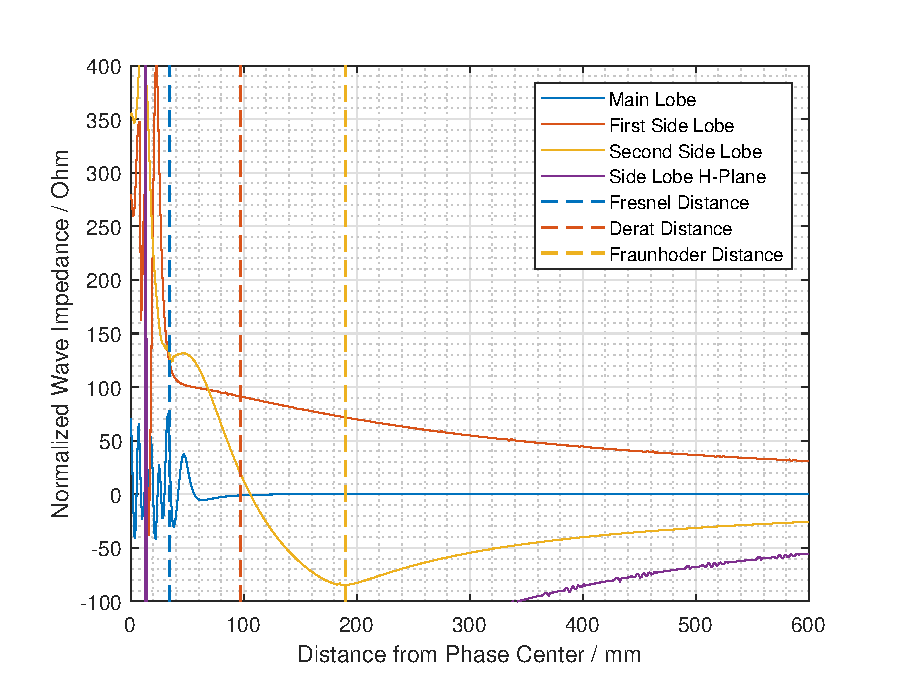
\includegraphics[width=0.49\textwidth]{Matlab/NormWaveImpHorn.eps}}
  \centering
  \subfigure[Phase]{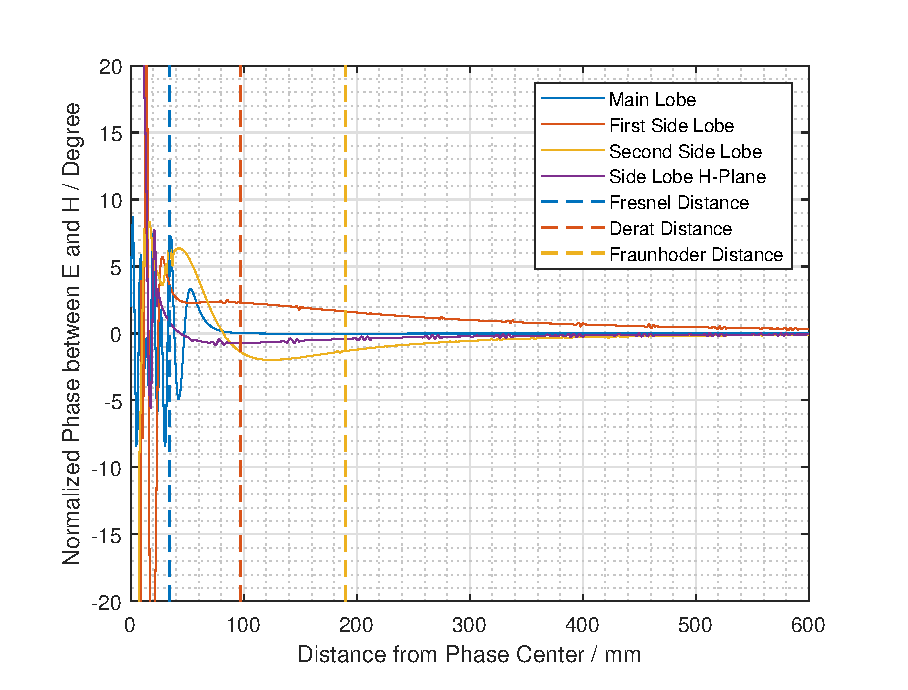
\includegraphics[width=0.49\textwidth]{Matlab/NormPhaseHorn.eps}}
  \centering
  \subfigure[EIRP]{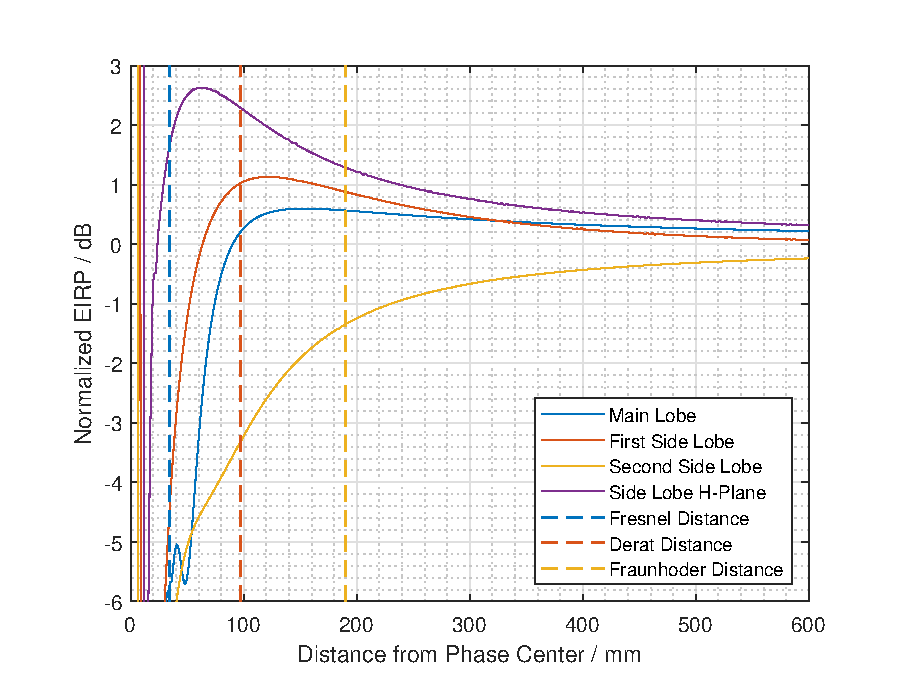
\includegraphics[width=0.49\textwidth]{Matlab/NormEIRPHorn.eps}}
  \centering
  \subfigure[Antenna Pattern E-Plane]{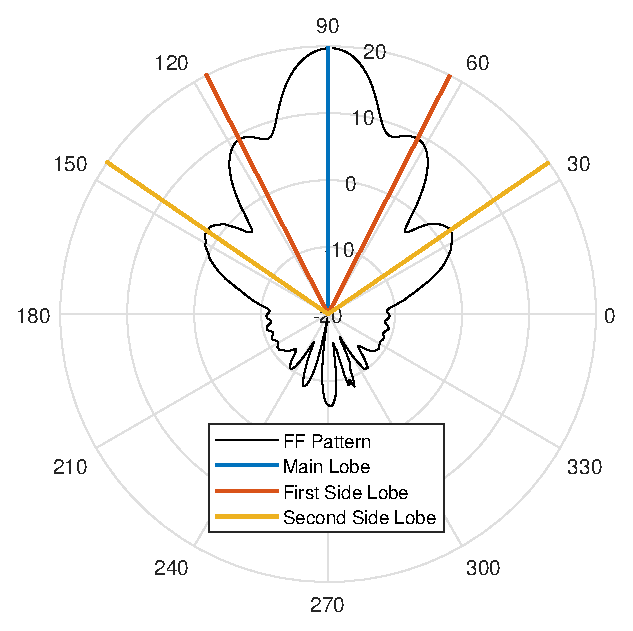
\includegraphics[width=0.35\textwidth]{Matlab/ePlanePattern.eps}}
\caption{Beam comparison of a $\SI{20}{\decibel}$ SGH at $\SI{28}{\giga\hertz}$}
\label{fig:beamcpmp}
\end{figure}

To clarify the introduced distances they will be proved based on a $\SI{20}{\decibel}$ \ac{SGH} at $\SI{28}{\giga\hertz}$. If you look in the annex at figure \ref{fig:fielddist} you see the front view of this horn with the underlying field distribution. The polarisation is in $y$-direction, so the $yz$-plane is called E-plane and the $xz$-plane is called H-plane from here on.\\
In figure \ref{fig:beamcpmp} the normalized wave impedance (a) and the normalized phase between E- and H-field components over the distance to the phase center are plotted. To clarify the designations the directions are plotted in (d). The data have been generated by CST\texttrademark , a full wave simulation tool. Complex data in $x$, $y$, and $z$ direction was exported and post processed to Matlab\texttrademark{}.\\
Also the field boundaries from the sections above are plotted with dashed lines. For deriving the boundaries only the opening of the horn in the E-plane was taken to account. This makes sense because the field distribution and thus the usage of the aperture is known, refer to figure \ref{fig:fielddist}. As you can see in the E-plane the aperture is fully used. But if the field distribution is unknown the smallest circle enclosing the aperture has to be taken.\\
In figure \ref{fig:beamcpmp} (a) the normalized wave impedance of the different angels (refer to (c)) is plotted over the distance from the antennas phase center. Figure \ref{fig:beamcpmp} (b) shows analogue to (a) the phase between E- and H-field.\\
The main lobe (blue line) is from Derat-distance on in \ac{FF} condition. On the one hand the wave impedance reached its end value of $\SI{377}{\ohm}$ and on the other hand E- and H-fields are coherent. Considering the side lobes it can be seen that in the reactive \ac{NF} the field conditions are very unstable, whereas the fields in the radiating \ac{NF} become more stable. In the \ac{FF} the field values are continually decreasing the offset from their final value.\\
In figure \ref{fig:devantennap} in the annex the resulting antenna patterns in different radii are depicted as well in Cartesian coordinates (a) as in Polar coordinates (b). The assumption 

\begin{equation}
S = \frac{E^2}{Z_0}
\label{eq:poynting}
\end{equation}

was taken to account. In addition analogue to (a) and (b) in (c) the \ac{EIRP} computed in different radii is plotted. At Derat distance ($\approx\SI{100}{\milli\meter}$) the error in main beam direction is about $\SI{0.5}{\decibel}$ and the antenna pattern is further evolving after the Fraunhofer distance at about $\SI{200}{\milli\meter}$.

\section{Spatial Sampling Approaches}

\begin{figure}[h]
\centering
\def\svgwidth{0.4\textwidth}
\input{Bilder/KoordinateSystem.pdf_tex}
\caption{The underlying coordinate system}
\label{coordinates}
\end{figure}

In figure \ref{coordinates} the used coordinate system is depicted. In comparison with a globe the latitude is described by the elevation with the symbol $\Theta$ and the longitude is described by the azimuth with the symbol $\Phi$. The value range of $\Theta$ and $\Phi$ is:

\begin{equation}
-\frac{\pi}{2} \leq \Theta <\frac{\pi}{2}\, ,\quad -\pi \leq \Phi < \pi
\end{equation}

Hereinafter different spatial sampling approaches for this sphere are introduced. For the development of a sampling grid a sampling frequency is necessary and will be introduced in the next section.

\subsection{Derivation of the Spatial Sampling considering the Array Factor}
\label{sec:spasa}

The \ac{AF} is \glqq the radiation pattern of an array antenna when each array element is considered to radiate isotropically\grqq{} \cite{ieeeantenna}. The sampling frequency in either elevation or in azimuth is dependent on the aperture of the \ac{DUT} and the wavelength. To investigate the necessary sampling frequency an one dimensional $\sfrac{\lambda}{2}$ array of isotropic radiators was taken in account. With the number of elements $N$, the element spacing $d = \sfrac{\lambda}{2}$ and the wavelength $\lambda$ the antenna pattern is derivable: \cite{litze}

\begin{equation}
\begin{vmatrix}\Gamma\left(\theta\right)\end{vmatrix}^2 = \Biggl|\frac{\sin\left(\frac{\pi M d}{\lambda \sin\left(\theta\right)}\right)}{\sin\left(\frac{\pi d}{\lambda \sin\left(\theta\right)}\right)}\Biggl|^2 = \Biggl|\frac{\sin\left(\frac{\pi M}{2 \sin\left(\theta\right)}\right)}{\sin\left(\frac{\pi}{2 \sin\left(\theta\right)}\right)}\Biggl|^2
\end{equation}

\begin{figure}[h]
  \centering
  \subfigure[Two elements: Pattern]{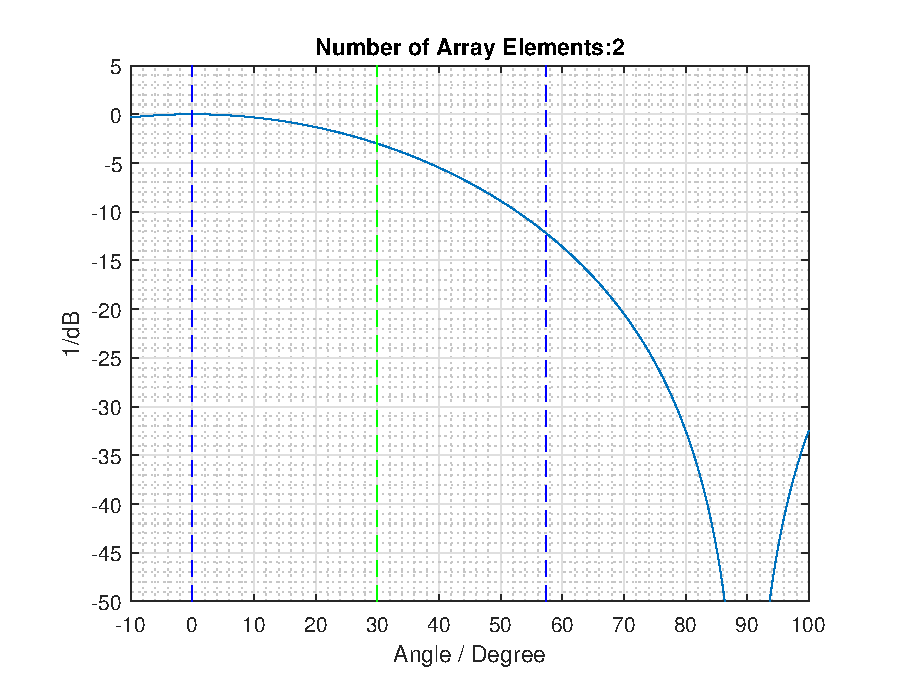
\includegraphics[width=0.32\textwidth]{Matlab/NoNumEl2.eps}}
  \centering
  \subfigure[Six elements: Pattern]{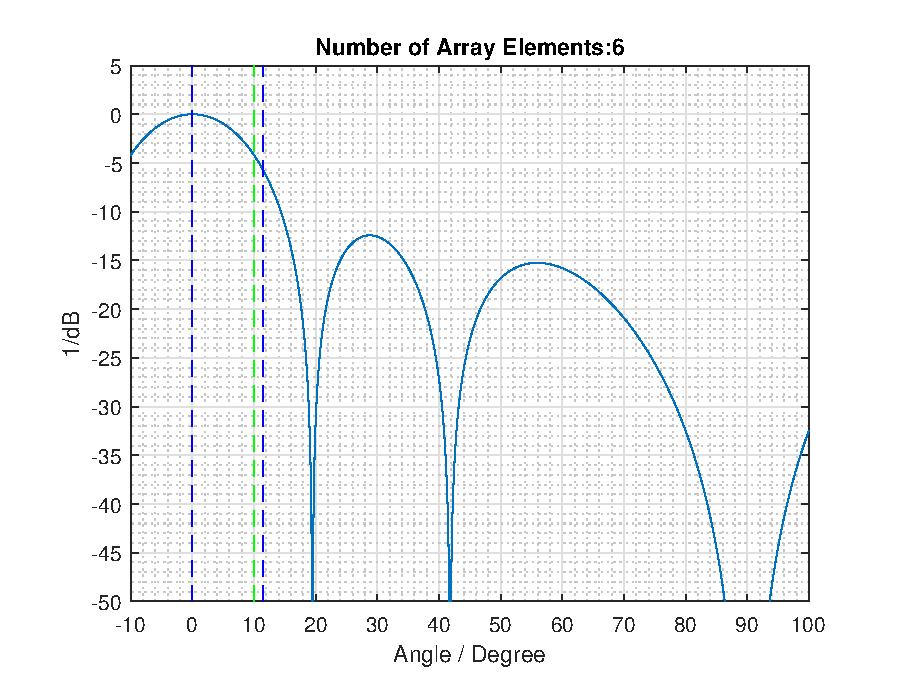
\includegraphics[width=0.32\textwidth]{Matlab/NoNumEl6.eps}}
  \centering
  \subfigure[100 elements: Pattern]{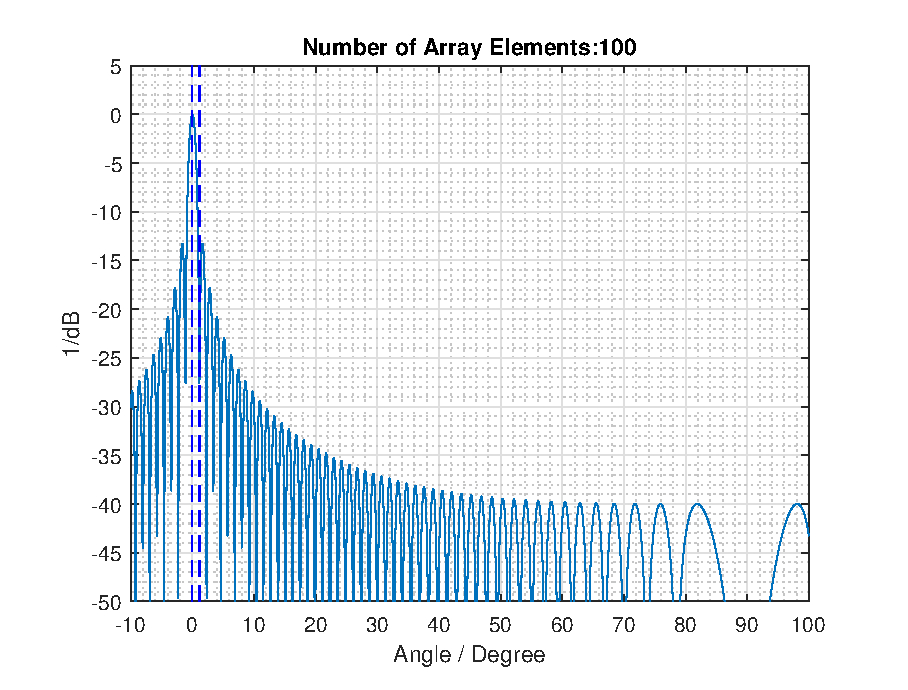
\includegraphics[width=0.32\textwidth]{Matlab/NoNumEl100.eps}}
\caption{Pattern of $N$-element array with $\sfrac{\lambda}{2}$-spacing}
\label{fig:evolvpattern2}
\end{figure}

\begin{figure}[h]
  \centering
  \subfigure[Two elements: Mode spectra]{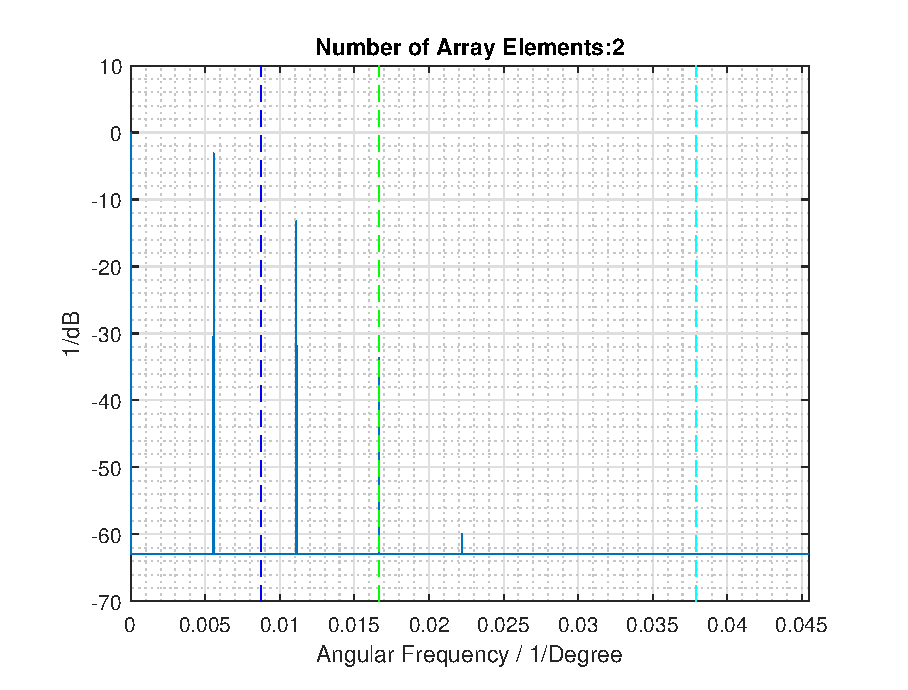
\includegraphics[width=0.32\textwidth]{Matlab/SpNumEl2.eps}}
  \centering
  \subfigure[Six elements: Mode spectra]{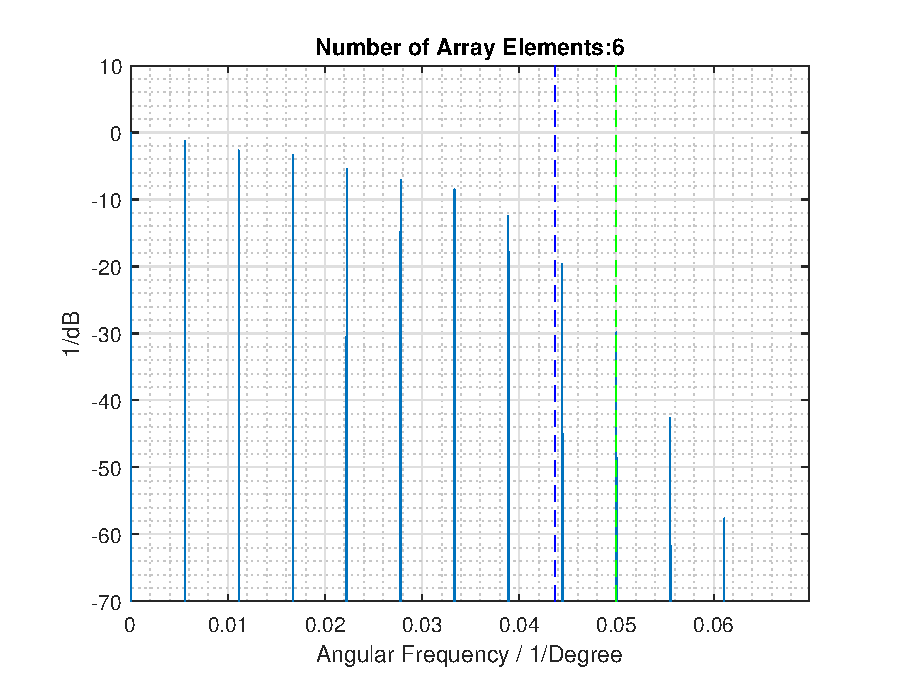
\includegraphics[width=0.32\textwidth]{Matlab/SpNumEl6.eps}}
  \centering
  \subfigure[100 elements: Mode spectra]{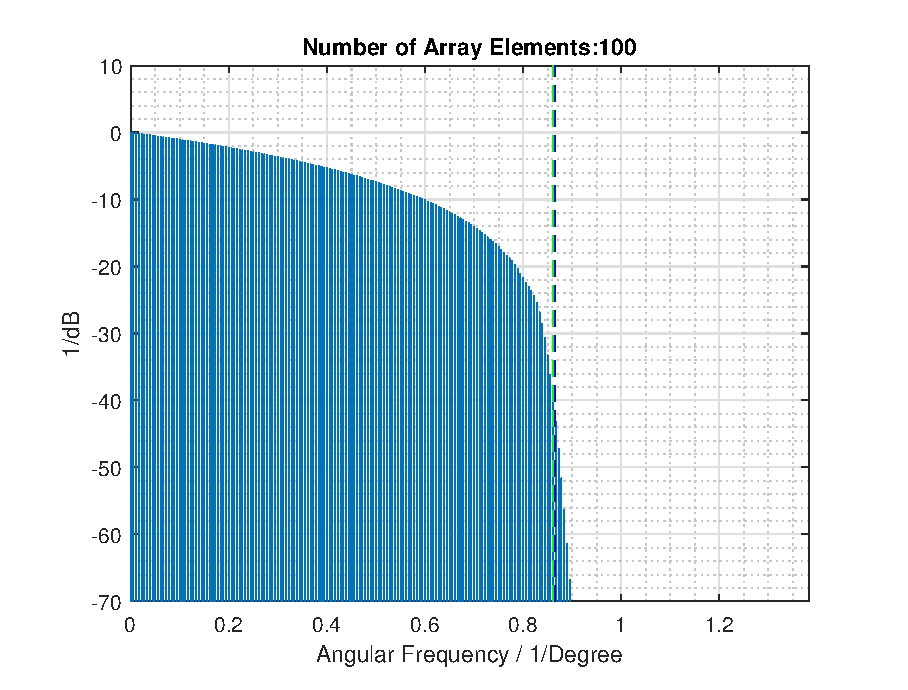
\includegraphics[width=0.32\textwidth]{Matlab/SpNumEl100.eps}}
\caption{Mode spectra of $N$-element array with $\sfrac{\lambda}{2}$-spacing}
\label{fig:evolvpattern3}
\end{figure}

The resulting pattern is depicted in figure \ref{fig:evolvpattern2} and in annex \ref{fig:evolvpattern} (a little larger).\\
In \cite{hansen} it is suggested to use the sampling increment of:

\begin{equation}
\Delta\Theta_\text{Hansen} = \frac{2\pi}{2N+1}\ , \quad \Delta\Phi_\text{Hansen}=\frac{2\pi}{2M+1}
\end{equation}

Where $N$ is the highest significant wave mode on the minimum sphere enclosing the antennas aperture and $M$ is the highest significant wave mode on the minimum cylinder. With the sphere radius $r_S$, the cylinder radius $r_C$ and the angular wavenumber $k = \sfrac{2\pi}{\lambda}$ they are calculated as follows:

\begin{equation}
N = kr_S+10\ , \quad M = kr_C+10
\end{equation}

For example, the resulting formula for the elevation is:

\begin{equation}
\Delta\Theta_{\text{ref}} = \lim_{r_S \to \infty}\Delta\Theta' = \lim_{r_S \to \infty} \frac{2\pi}{2\left(kr_S+10\right)+1} = \frac{\lambda}{2\cdot r_S}
\end{equation}

And the azimuth is:

\begin{equation}
\Delta\Phi_{\text{ref}} = \frac{\lambda}{2\cdot r_C}
\end{equation}

These angle increments were also introduced in \cite{2018arXiv180310993F} and are called reference angle increments. To illustrate these angle increments the one dimensional array of isotropic radiators is taken. Evaluating the \ac{AF} of a $d = \sfrac{\lambda}{n}$ -array with $N$ elements the reference angle becomes very short:

\begin{equation}
\Delta\Phi_{\text{ref}} = \frac{n}{N-1}
\label{eq:1dinc}
\end{equation}

With the \ac{FFT} over the angle of the antenna patterns from figure \ref{fig:evolvpattern2} the mode spectra can be derived and is seen in figure \ref{fig:evolvpattern3} (or \ref{fig:evolvpattern} in annex).\\
When an arbitrary signal is sampled, the spectrum is mirrored at the sampling frequency. Choosing a sampling frequency lower than twice the highest occurring frequency in the sampled signal causes an irreversible error. This is called the Nyquist-Shannon sampling theorem.\\
For that sake the dashed lines are:

\begin{equation}
\color{blue}\left(\Delta\Phi_{\text{ref}}\right)^{-1}\color{black},\ \color{cyan}\left(\Delta\Phi_\text{Hansen}\right)^{-1}\color{black}\ \text{and}\ \color{green}\text{first mode} > \SI{-40}{\decibel} \color{black}
\end{equation}

Similar to that the dashed lines in figure \ref{fig:evolvpattern2} are the first sampling points using the derived sampling frequency.\\
The issue is now to find the sampling frequency at which the sampling error is independent from the aperture of the antenna. As depicted in figure \ref{fig:evolvpattern3} the sampling frequency introduced by \cite{hansen} is too strict for small apertures. On the other hand the reference angle introduced by \cite{2018arXiv180310993F} is to inaccurate for small apertures. Because of that a new factor \ac{CrefA} is taken:

\begin{equation}
\text{CrefA} = \left(\Delta\Phi_{\text{ref}}\cdot\left(\text{first mode} > \SI{-40}{\decibel}\right)\right)^{-1}
\end{equation} 

\begin{figure}
\centering
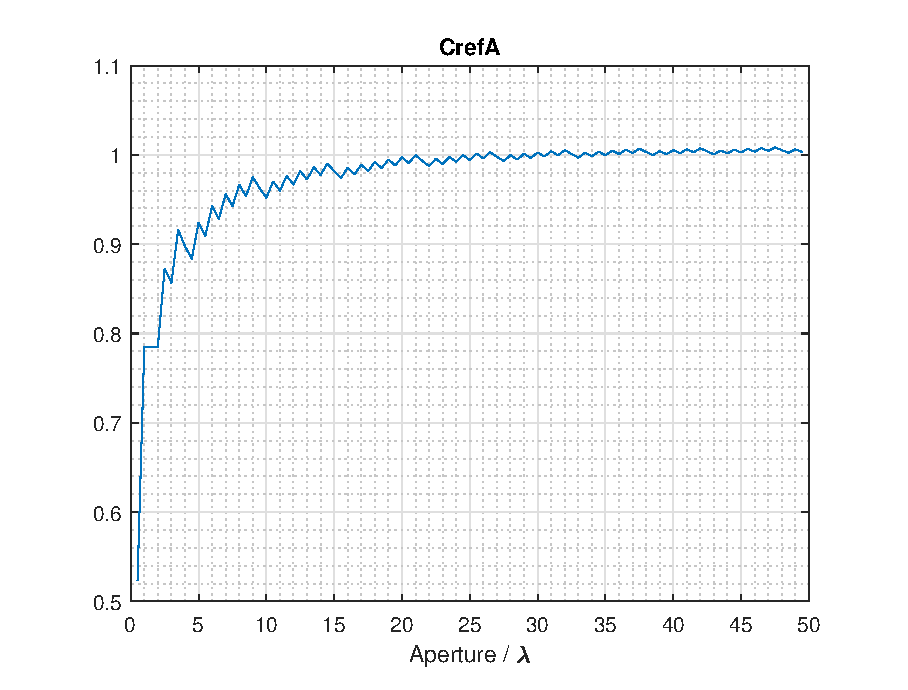
\includegraphics[width=0.41\textwidth]{Matlab/CrefA.eps}
\caption{Correction Factor Reference Angle}
\label{fig:crefa}
\end{figure}

This factor is plotted in figure \ref{fig:crefa}. It is dependent of the aperture. With that the error due to sampling is independent from the antennas aperture. Less than $\SI{-40}{\decibel}$ in the mode spectra is defined for the sampling angle increment in \cite{hansen}.\\
For further reduction of points a second factor is introduced, the \acf{SF}. At $\text{SF}=2$ every second measurement point is skipped. With all that the angle increments for spherical sampling is:

\begin{equation}
\Delta\Theta = \text{SF}\cdot\text{CrefA}\left(\sfrac{2r_S}{\lambda}\right)\cdot\frac{\lambda}{2r_S}\ ,\quad\Delta\Phi = \text{SF}\cdot\text{CrefA}\left(\sfrac{2r_C}{\lambda}\right)\cdot\frac{\lambda}{2r_C}
\label{eq:angle}
\end{equation}

\subsection{Constant Step Size Grid}


\begin{figure}[h]
  \centering
  \subfigure[independent azimuth step size]{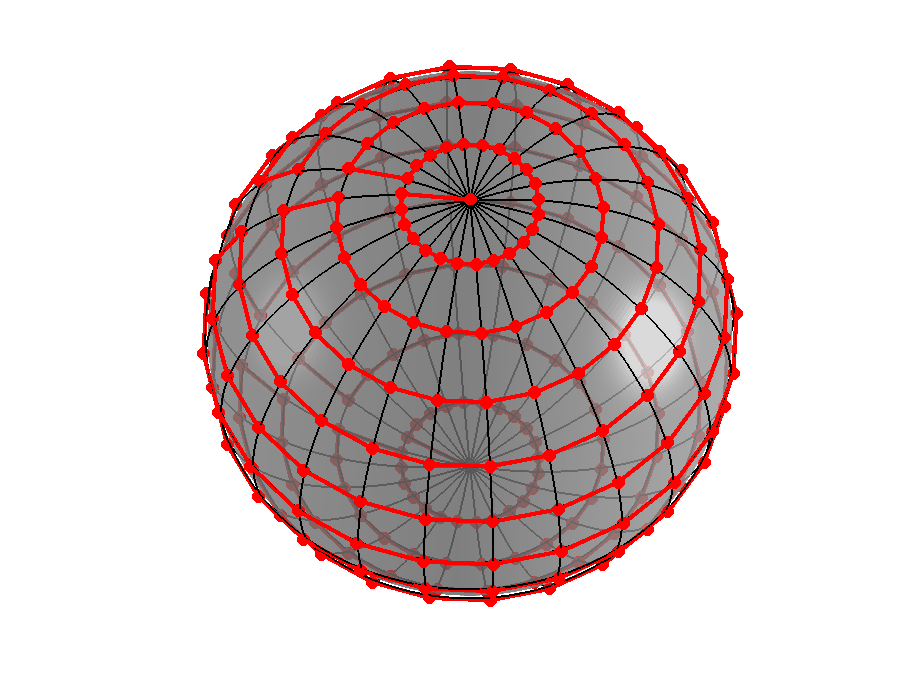
\includegraphics[width=0.49\textwidth]{Matlab/GridCoStPolar.eps}}
  \centering
  \subfigure[dependent azimuth step size]{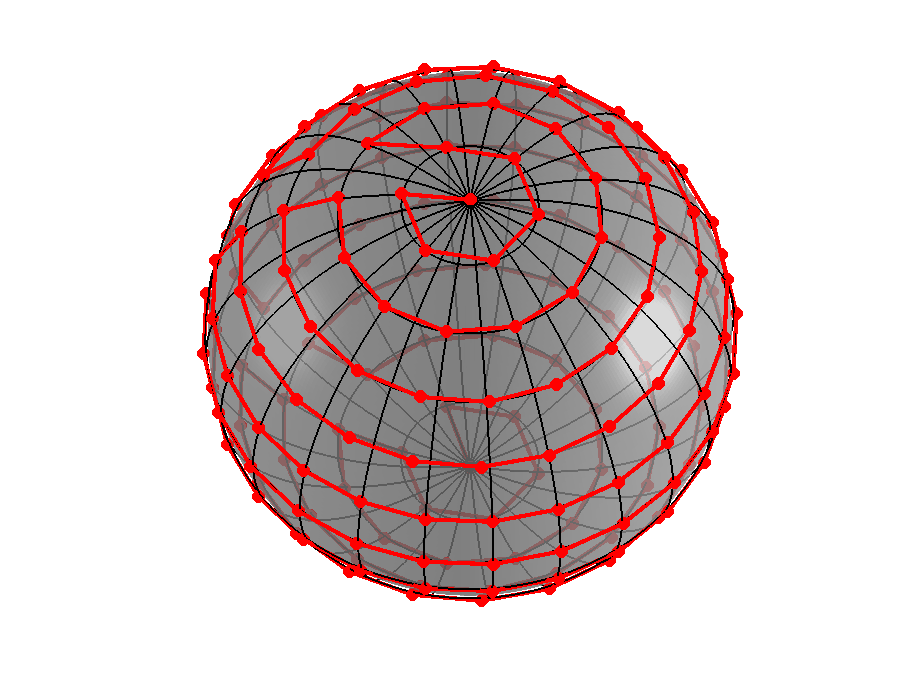
\includegraphics[width=0.49\textwidth]{Matlab/GridCoStSinPolar.eps}}
\caption{$\SI{15}{\degree}$ -Constant Step Size Grid}
\label{fig:cssg}
\end{figure}

The most straight forward way to a spherical measurement is using a \ac{CSSG} depicted in figure \ref{fig:cssg} (a). The advantage is the easy feasibility with any positioner. Ether the azimuth can be swept on every latitude circle or the elevation can be swept on every longitude circle. On the other hand the measurement density is higher on the poles than on the equator.\\
To meet that the theta dependent number of azimuth points was introduced e.g. by \cite{ctiaat}. It is applied as follows:

\begin{align}
N_{\text{max}} = \frac{2\pi}{\Delta\Phi}\\
N\left(\Theta\right)=\lceil N_{\text{max}}\cdot\cos\left(\Theta\right)\rceil\\
\Delta\Phi\left(\Theta\right) = \frac{2\pi}{N\left(\Theta\right)}
\end{align}

It is only possible to sweep the azimuth when this type of grid is used. For easier reviewing, the grid is also plotted in Certesian coordinates in figure \ref{fig:gridcomp} in the annex. The red line is a suggested sequence.

\subsection{Constant Density}

\begin{figure}[h]
  \centering
  \subfigure[Polar Coordinates]{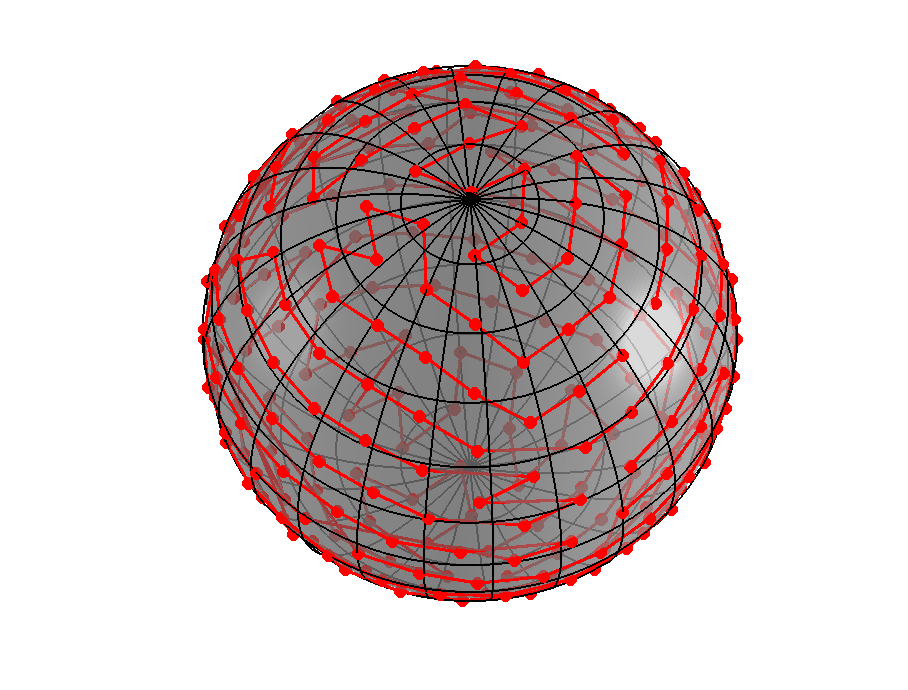
\includegraphics[width=0.49\textwidth]{Matlab/GridCoDePolar.eps}}
  \centering
  \subfigure[Cartesian Coordinates]{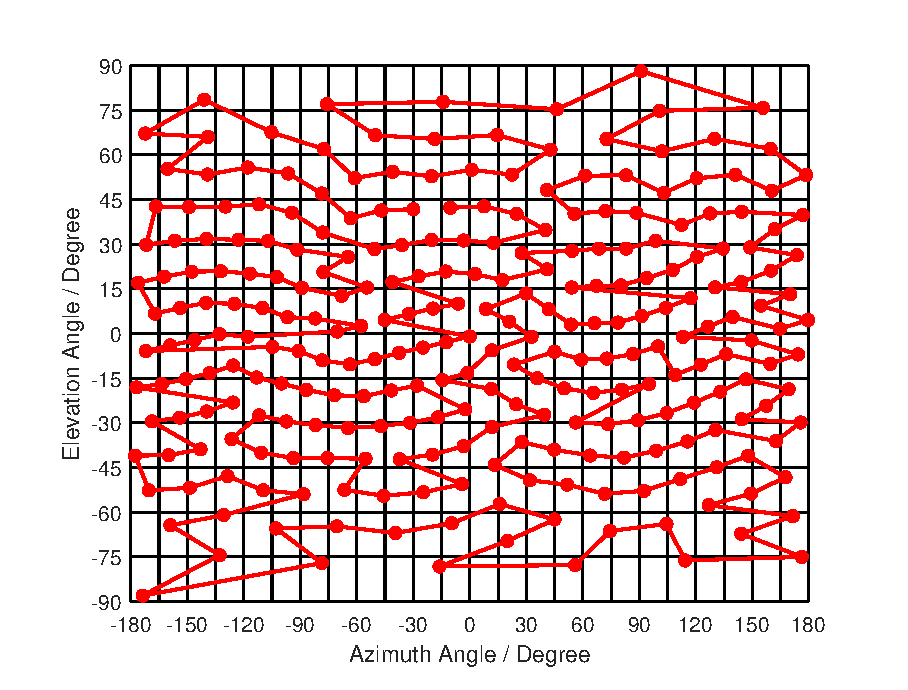
\includegraphics[width=0.49\textwidth]{Matlab/GridCoDeCart.eps}}
\caption{Constant Density Grid with 264 Measurement points}
\label{fig:cdg}
\end{figure}

The \ac{CDG} depicted in figure \ref{fig:cdg} was produces and generated by a charged particle algorithm. It works by minimising the cumulated potential energy of all measurement dots considered as charged particles. The potential energy is minimal, when all points are evenly distributed over the sphere.\\ 
Deriving the optimal measurement sequence is a \ac{TSP}. It is solved by the Matlab toolbox introduced in \cite{tsp} viewing the angles as Cartesian coordinates. This path is optimized for the positioner to move as efficient as possible. Because the positioning in Azimuth is faster than in Elevation, the elevation distance is weighted five times more. Furthermore the periodicity is taken to account, so that the distance between tow points $\text{P}_n$ and $\text{P}_m$ is:

\begin{equation}
\Delta\Theta_{mn} = 5\left(\Theta_{\text{P}_n}-\Theta_{\text{P}_m}\right)\ ,\quad \Delta\Phi_{mn} = \text{min}\left(|\Phi_{\text{P}_n}-\Phi_{\text{P}_m}|\, ,\ 2\pi-|\Phi_{\text{P}_n}-\Phi_{\text{P}_m}|\right)
\end{equation}

With that the quadratic distance Matrix $D$ can be derived using euclidean distance with $d_{mn} = \sqrt{\Delta\Theta_{mn}^2+\Delta\Phi_{mn}^2}$ out of $N$ Points:

\begin{equation}
D = \begin{bmatrix}
 0 & d_{12} & \dots & d_{1N}\\
 d_{21} & 0 & \dots & d_{2N}\\
 \vdots & \vdots & \ddots & \vdots\\
 d_{N1} & d_{N2} & \dots & 0
\end{bmatrix}
\end{equation}

The cumulated distance for $N = 264$ is converged after around one million iterations. The result is depicted in figure \ref{fig:cdg} (b).

\subsection{Other}

There are other grid types, which are mainly based on the already introduced grids. First there are Cardinal cuts, here a measurement is carried out along the equator and one, tow or more orthogonal meridians. If the alignment is right a technique called \acf{PM} can be used to calculate the complete antenna pattern out of the cardinal cuts. The problem here is that a symmetry is assumed which is always wrong if the direction of main beam and the orientation of the pattern is unknown. \cite{2018arXiv180310993F}\\
An other spatial sampling approach is the Spiral Scan. It is developed by \ac{RS} and can be used for a pre scan to find the maximum \ac{EIRP} direction. Here elevation and azimuth is swept. \cite{ctiaat}

\section{Total Radiated Power Quadratures}
\label{sec:quadrature}

The easiest way to derive the \ac{TRP} is if Cardinal cuts or a \ac{CDG} was taken, to compute the mean of all \ac{EIRP} samples. For other grids the quadrature needs to be done as follows. \cite{trp}

\subsection{Sine Theta}

The straight forward way is to transform the integral over a spherical surface $S$

\begin{equation}
\text{TRP} = \frac{1}{4\pi}  \oiint_S \text{EIRP}\left(\theta,\phi\right)\cdot\sin\theta\cdot d\theta d\phi
\label{eq:trpint}
\end{equation}

to a sum, this is called quadrature. The easiest approach is carried out by discretizing the integral Argument:  \cite{ctiaat}

\begin{equation}
\frac{1}{4\pi}\cdot\sin\theta\cdot d\theta\cdot d\phi \ \Rightarrow\ \frac{1}{4\pi}\cdot \Delta\theta\cdot \Delta\phi\cdot\sin\theta = \frac{1}{4\pi}\cdot \frac{\pi}{N}\cdot \frac{2\pi}{M}\cdot\sin\theta=\frac{\pi}{2NM}\cdot\sin\theta
\end{equation}

With that the quadrature is:

\begin{equation}
\text{TRP}_{\sin\theta} = \frac{\pi}{2NM}\sum^{N-1}_{i=1}\sum^{M-1}_{j=0}\left(\text{EIRP}_\theta\left(\theta_i,\phi_j\right)+\text{EIRP}_\phi\left(\theta_i,\phi_j\right)\right)\cdot\sin\left(\theta_i\right)
\label{eq:trpsumsin}
\end{equation}

$N$ is the number of angular intervals in $\theta=\left[0,\pi\right]$ (elevation), $M$ is the number of angular intervals in $\phi=\left[0,2\pi\right]$ (azimuth), the indices $i=\left[0,N\right]$, $j=\left[0,M\right]$ and the \ac{EIRP} is split in its horizontal ($\text{EIRP}_\phi$) and its vertical ($\text{EIRP}_\theta$) part. This quadrature is called sine theta.

\subsection{Clenshaw-Curtis}

Because the sine theta quadrature is not accurate for spars measurements and the measurement points at the poles are neglected, an other weighting scheme is used, the \ac{CC}-quadrature. For the sine theta quadrature the integrating surface is constantly interpolated (compare equation \ref{eq:trpsumsin}). The \ac{CC} quadrature is more accurate using the weights W computed by expending the integrand with Chebyshev polynomials. With that formula \ref{eq:trpsumsin} develops to: \cite{trp}

\begin{equation}
\text{TRP}_{\text{CC}} = \frac{1}{2M}\sum^{N-1}_{i=1}\sum^{M-1}_{j=0}\left(\text{EIRP}_\theta\left(\theta_i,\phi_j\right)+\text{EIRP}_\phi\left(\theta_i,\phi_j\right)\right)\cdot\text{W}\left(\theta_i\right)
\label{eq:trpsumcc}
\end{equation}

\subsection{Jacobi}

The Jacobi quadrature uses the area of triangles on the spherical surface between the measurement points. The average \ac{EIRP} of a triangle is computed and weighted by the area $A_i$ of it. The result is normed with the complete surface area. With that for every triangle $i=\left[1,N\right]$ the \ac{TRP} quadrature is: \cite{trp}

\begin{equation}
\text{TRP}_{\text{J}} = \frac{\sum^N_{i=1}A_i\left(\frac{\text{EIRP}_{0,i}+\text{EIRP}_{1,i}+\text{EIRP}_{2,i}}{3}\right)}{\sum^N_{i=1}A_i}
\end{equation}

\subsection{Comparing the Quadratures}

Sine Theta- and \ac{CC} quadratures are only applicable for \acp{CDG} and with slight optimizations also for \acp{CDG} with less dense measurements at the poles. Whereas the Jacobi quadrature can be used for arbitrary grids.\\
In \cite{trp2} it is investigated which quadrature leads to the most accurate result with the same number of points. The result is that \ac{CC}- and Jacobi quadratures are equally accurate.

\section{Statistics and Regression}

This section shall give a brief introduction in the field of statistics and regression, which is necessary for the spatial sampling simulation. First statistical terms, than methods to display scatterings and multidimensional regressions are introduced.

\subsection{Metrics to Describe Distributions}

To describe a one dimensional scattering $h$ with $N$ samples $x$ and the cumulative frequency $H$, these terms are regularly used: \cite{dffs}

\begin{itemize}
\item The commonly most used and known term s the \textbf{Arithmetic Mean}, which is vulnerable by outliers and computed as:
\begin{equation}
\bar x = \frac{1}{N}\sum_{n=1}^N x_N
\end{equation}
\item The \textbf{Median} is that value lying in the middle of a distribution, so that $H\left( x\right) = 0.5$. It is computed by sorting the samples by value and, if the number of samples is even, taking the mean of the two samples in the middle, or if the number of samples is odd taking the middle value.
\item The \textbf{Variance} of a distribution is the sum of squared error, normalized by the number of samples. This metric is strongly vulnerable by outliers. The computation is as follows:
\begin{equation}
s^2 = \frac{1}{N-1}\sum_{n=1}^N\left( x_n-\bar{x}\right)^2
\end{equation}
\item The \textbf{$p$-Quantile} is analogue to the Median, that value of a sorted sample vector where $P$ percent of the distributions values is reached, hence $H\left( x\right) = p$.
\item A more stable metric for scattering as the variance is the \textbf{\ac{IQR}}, this describes the range between two quantiles.
\end{itemize}

\subsection{Display a Distribution}

The commonly known way to display a distribution is a bar diagram. There the value of range is split in $M$ bars displaying the values in the $x$-axis and the probability of each bucket on the $y$-axis. An other way to display a distribution is the box-plot, where only the minimal, maximal, $\SI{25}{\percent}$-quantile, median and $\SI{75}{\percent}$-quantile value is plotted.

\subsection{Distribution Functions}
There are all sorts of scattering distributions e.q. even distribution, Weibull distribution, Rayleigh distribution, ... but the most prominent distribution is the normal distribution by Gauss:

\begin{equation}
f\left( x \right) = \frac{1}{\sigma\sqrt{2\pi}}e^{-\frac{1}{2}\left(\frac{x-\mu}{\sigma}\right)^2}
\end{equation}

Assuming that $\sigma = s$ and $\mu = \bar{x}$ this function can also be plotted and used for predictions.

\subsection{Regression of multidimensional Datasets}
\label{sec:regod} 
Assuming a input variable vector $\vec{x}$, a coefficient set $\vec{b}$ and a result $y$ an arbitrary polynomial can be written as: \cite{sip}

\begin{equation}
y\left(\vec{x}\right) = \vec{x}^{\mathsf T}\cdot\vec{b}=\begin{bmatrix}
1 & x_1 & x_2 & \dots & x_M
\end{bmatrix} \cdot \begin{bmatrix}
b_0 \\ b_1 \\ b_2 \\ \vdots \\ b_M
\end{bmatrix}
\end{equation}

With $N$ samples this system is overdetermined which leads to an error vector $\vec{e}$. Than the resulting polynomial is:

\begin{equation}
\vec{y}=X\cdot \vec{b}+\vec{e}=\begin{bmatrix}
y_1 \\ y_2 \\ \vdots \\ y_N
\end{bmatrix} = \begin{bmatrix}
1 & x_{11} & x_{12} & \dots & x_{1M} \\
1 & x_{21} & x_{22} & \dots & x_{2M} \\
\vdots & \vdots & \vdots & \ddots & \vdots \\
1 & x_{N1} & x_{N2} & \dots & x_{NM}
\end{bmatrix} \cdot \begin{bmatrix}
b_0 \\ b_1 \\ b_2 \\ \vdots \\ b_M
\end{bmatrix} + \begin{bmatrix}
e_1 \\ e_2 \\ \vdots \\ e_N
\end{bmatrix}
\end{equation}

The sum square error

\begin{equation}
S = \vec{e}^{\mathsf T}\cdot\vec{e}=\left(\vec{y}-X\cdot\vec{b}\right)^{\mathsf T}\cdot\left(\vec{y}-X\cdot\vec{b}\right)
\end{equation}

is minimized by 

\begin{equation}
\nabla_{\vec{b}}\cdot S = 0
\end{equation}

leading to the well known \ac{LS}-method

\begin{equation}
\hat{b}_\text{LS}=\left(X^{\mathsf T} X\right)^{-1} X^{\mathsf T}\vec{y}.
\end{equation}

The input matrix $X$ can also be optimized by taking combinations or powers of different dependent parameters.\\
A frequent problem is that the significance of the parameters in $\vec{b}$ is unknown, hence to unnecessary high number of parameters and inaccurate regressions. Therefore the hypothesis that $b_m=0$ is checked. The parameters in vector $\vec{b}$ are t-distributed. First the covariance matrix of the independent variable $\vec{y}$ is estimated: \cite{dffs}

\begin{equation}
C = \left(X^{\mathsf T} X\right)^{-1}\frac{1}{N-M-1}\cdot\left(\vec{y}^{\mathsf T}\cdot\vec{y}-\vec{b}^{\mathsf T}\cdot X^{\mathsf T}\cdot \vec{y}\right) = \begin{bmatrix}
c_{00} & c_{01} & \dots & c_{0M} \\
c_{10} & c_{11} & \dots & c_{1M} \\
\vdots & \vdots & \ddots & \vdots \\
c_{M0} & c_{M1} & \dots & c_{MM}  
\end{bmatrix}
\end{equation}

With the variances $c_{mm}$ of each parameter and the variance of $\vec{y}$ $s$, the $p$-value can be computed with $F_t$, the \ac{CDF} of the t-distribution with $N-1$ degrees of freedom:

\begin{equation}
p_m = F_t\left(\frac{b_m}{c_{mm}\cdot s}\right)
\end{equation}

Normally a significance value of $\alpha = \SI{5}{\percent}$ is chosen. If the $p$-value is inside the interval $p_m=\left[\sfrac{\alpha}{2},\ 1-\sfrac{\alpha}{2}\right]$ the hypothesis is valid and parameter $m$ can be discarded.

To estimate the confidence interval for the mean of a regression at a point $x_0$ the variance at dot $x_0$ must be estimated: \cite{dffs}

\begin{equation}
s_{\hat{y}_0}^2 = \frac{1}{N-M-1}\cdot\left(\vec{y}^{\mathsf T}\cdot\vec{y}-\vec{b}^{\mathsf T}\cdot X^{\mathsf T}\cdot \vec{y}\right)\cdot \vec{x}_0^{\mathsf T}\cdot \left(X^{\mathsf T} X\right)^{-1} \cdot \vec{x}_0
\end{equation}

Choosing a confidence value $\gamma = \SI{95}{\percent}$, the two parameters $k_1$ and $k_2$ can be derived with the inverse \ac{CDF} $F_t^{-1}$ with $N-M-1$ degrees of freedom:

\begin{equation}
k_1 = F^{-1}\left(\frac{1-\gamma}{2}\right),\ k_2 = F^{-1}\left(\frac{1+\gamma}{2}\right)
\end{equation}

And the confidence interval is:

\begin{equation}
\mu_y\left(\vec{x}_0\right) =\left[ y\left(\vec{x}_0\right)-k_2\cdot s_{\hat{y}_0},\ y\left(\vec{x}_0\right)-k_1\cdot s_{\hat{y}_0}\right]
\label{eq:conv}
\end{equation}


